\documentclass{templateNote}
\usepackage{tcolorbox}
\usepackage{amsmath}
\usepackage{amssymb}
\usepackage{pgfplots}
\usepackage{pgf-pie}
\usepackage{tabularx}
\usepackage[ruled,vlined]{algorithm2e}
\usepackage{soul}

\pgfplotsset{compat=1.18}
\newcolumntype{L}{>{\centering\arraybackslash}X}
\begin{document}

\imagenlogoU{img/LogoElNube.png}
\linklogoU{https://github.com/MarceloPazPezo}
\linkDoc{https://github.com/MarceloPazPezo/MyRepo/blob/main/Icinf/Semestre\%206/Analisis\%20y\%20Diseño\%20de\%20Algoritmos/ApunteC2/ApunteC2.pdf}
\universidad{Universidad del Bío-Bío}
\titulo{Apunte Certamen 2} % Titulo
\asignatura{Analisis y Diseño de Algoritmos} % Asignatura
\autor{
    Marcelo \textsc{Paz}
}
\portada
\margenes % Crear márgenes

\section{Importante}
\begin{itemize}
    \item \textbf{Backtracking:} Tipo de algoritmo que se utiliza para resolver problemas de satisfacción de restricciones (CSP).
    \item \textbf{Algoritmos Probabilísticos:} Son aquellos que introducen elementos al azar dentro de su lógica.
    
    Tipos de algoritmos probabilísticos:
    \begin{itemize}
        \item \textbf{Algoritmos Monte Carlo (Probable que mienta):} Da la respuesta exacta, pero puede dar una solución errada, con probabilidad baja (puede mentir).
        \item \textbf{Algoritmos Las Vegas (Probable que NO encuentre solución):} Funciona similar a Monte Carlo, pero cuando no puede dar una respuesta correcta, lo admite (no miente, dice que no puede dar la respuesta correcta).
        
        Se distinguen 2 sub-tipos en general:
        \begin{itemize}
            \item \textbf{Algoritmos de Sherwood:} Siempre encuentra una solución correcta. Si el azar no beneficia a la ejecución, esta tomará más tiempo.
            \item \textbf{Algoritmos que, a veces, no dan respuesta:} A veces no es capaz de dar una solución, lo cual admite.
        \end{itemize}
        
        \item \textbf{Algoritmos Genéticos:} Es una metaheurística que se inspira en la evolución y selección natural para resolver problemas de optimización, busca elegir al individuo más fuerte.
        
        \begin{itemize}
            \item \textbf{Fitness:} Función de aptitud, nos dice que tan apta es la solución para el problema (que tan cerca estamos de la solución real).
        \end{itemize}
        
        \item \textbf{Teoría de la Información:} Trata sobre clasificación de problemas, mide tiempo y espacio utilizando modelos de cómputo.
        \begin{itemize}
            \item \textbf{Entropía(mínimo teórico):} Mide la cantidad de información que tiene un mensaje.
            \begin{align*}
                h &=  \sum_{i=1}^{n} p_i \cdot \log_2 \left( \frac{1}{p_i} \right)
            \end{align*}
                
            \item \textbf{Kolmogorov(mínimo real):} Mide la cantidad de información que tiene un mensaje.
            \begin{align*}
                K &= \min \left\{ l(M) : U(M) = x \right\}
            \end{align*}
            Donde $l(M)$ es la longitud del mensaje y $U(M)$ es el programa que genera el mensaje $M$.
        \end{itemize}

        \item \textbf{Reducciones:} Son métodos para demostrar alguna característica de un problema.
        \begin{itemize}
            \item \textbf{Reducción Turing:} Es una reducción para demostrar que un problema es imposible de resolver, usando otro problema que ya se sabe que es imposible de resolver.
            Ejemplo:

            \begin{center}
                HP $\leq_T$ EP
            \end{center}
            Donde HP es el problema de parada y EP es el problema del vacío.
            \\
            \item \textbf{Reducción Karp:} Es una reducción para demostrar que un problema es difícil de resolver, usando otro problema que ya se sabe que es difícil de resolver.
            Ejemplo:

            \begin{center}
                3-SAT $\leq_p$ K-Clique
            \end{center}
            Donde 3-SAT es el problema de satisfacción de 3 variables y K-Clique es el problema de encontrar un clique de tamaño K.
            \\
        \end{itemize}
    \end{itemize}
    
    \textbf{Problema visto en clase:}
    \begin{figure}[H]
        \centering
        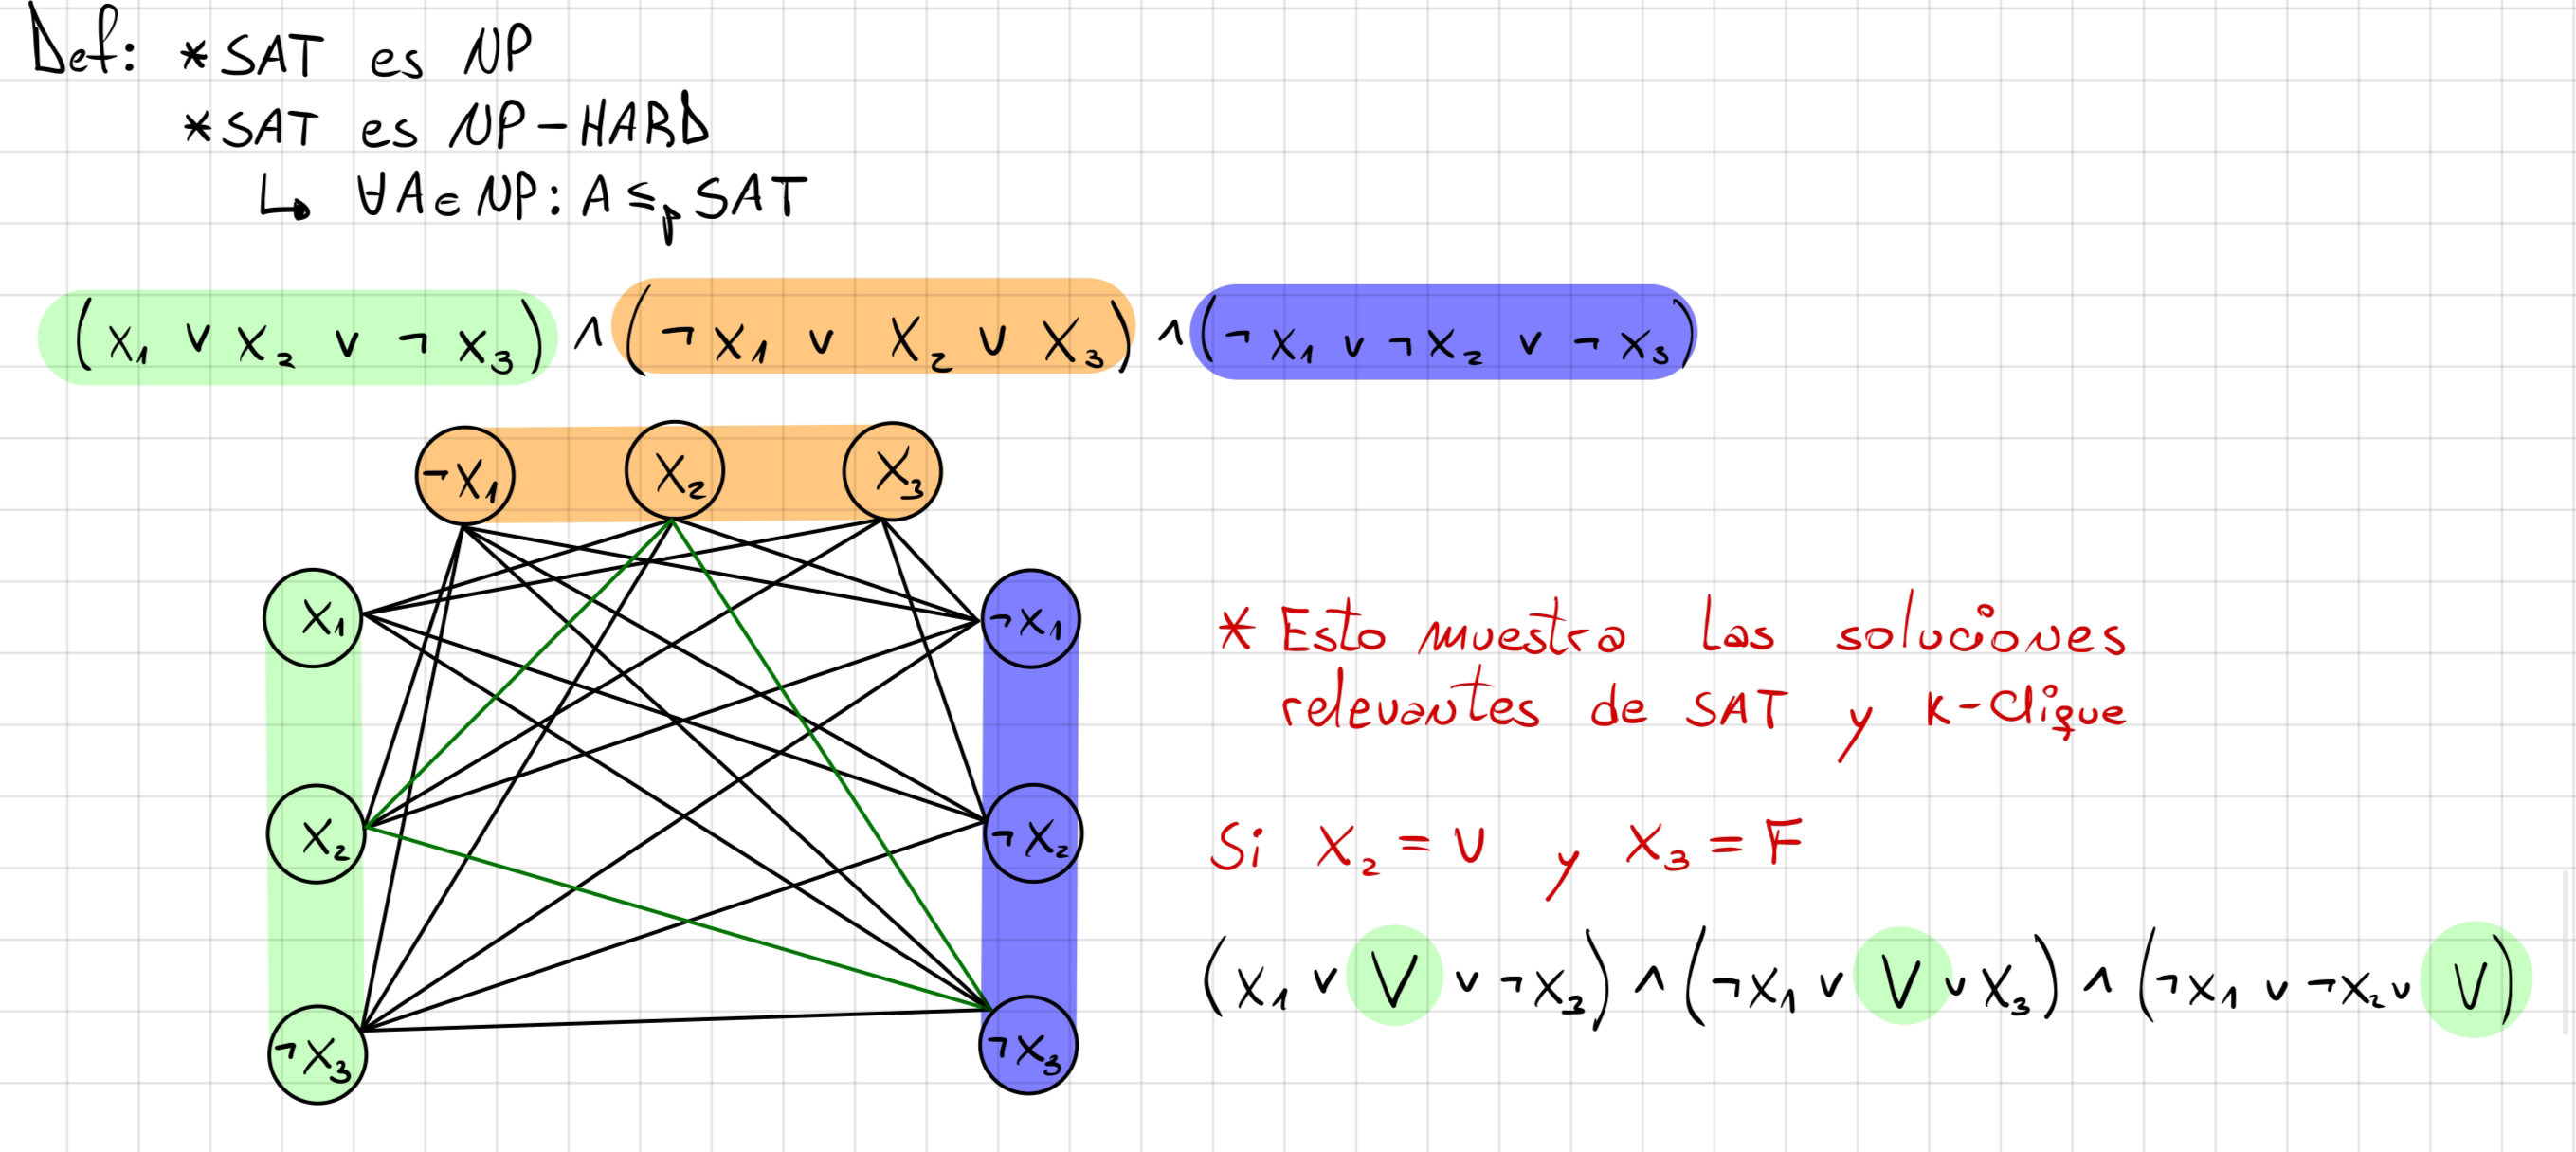
\includegraphics[scale=0.16]{img/Problema3-SATK-CliqueP1.jpeg}
    \end{figure}
    \begin{figure}[H]
        \centering
        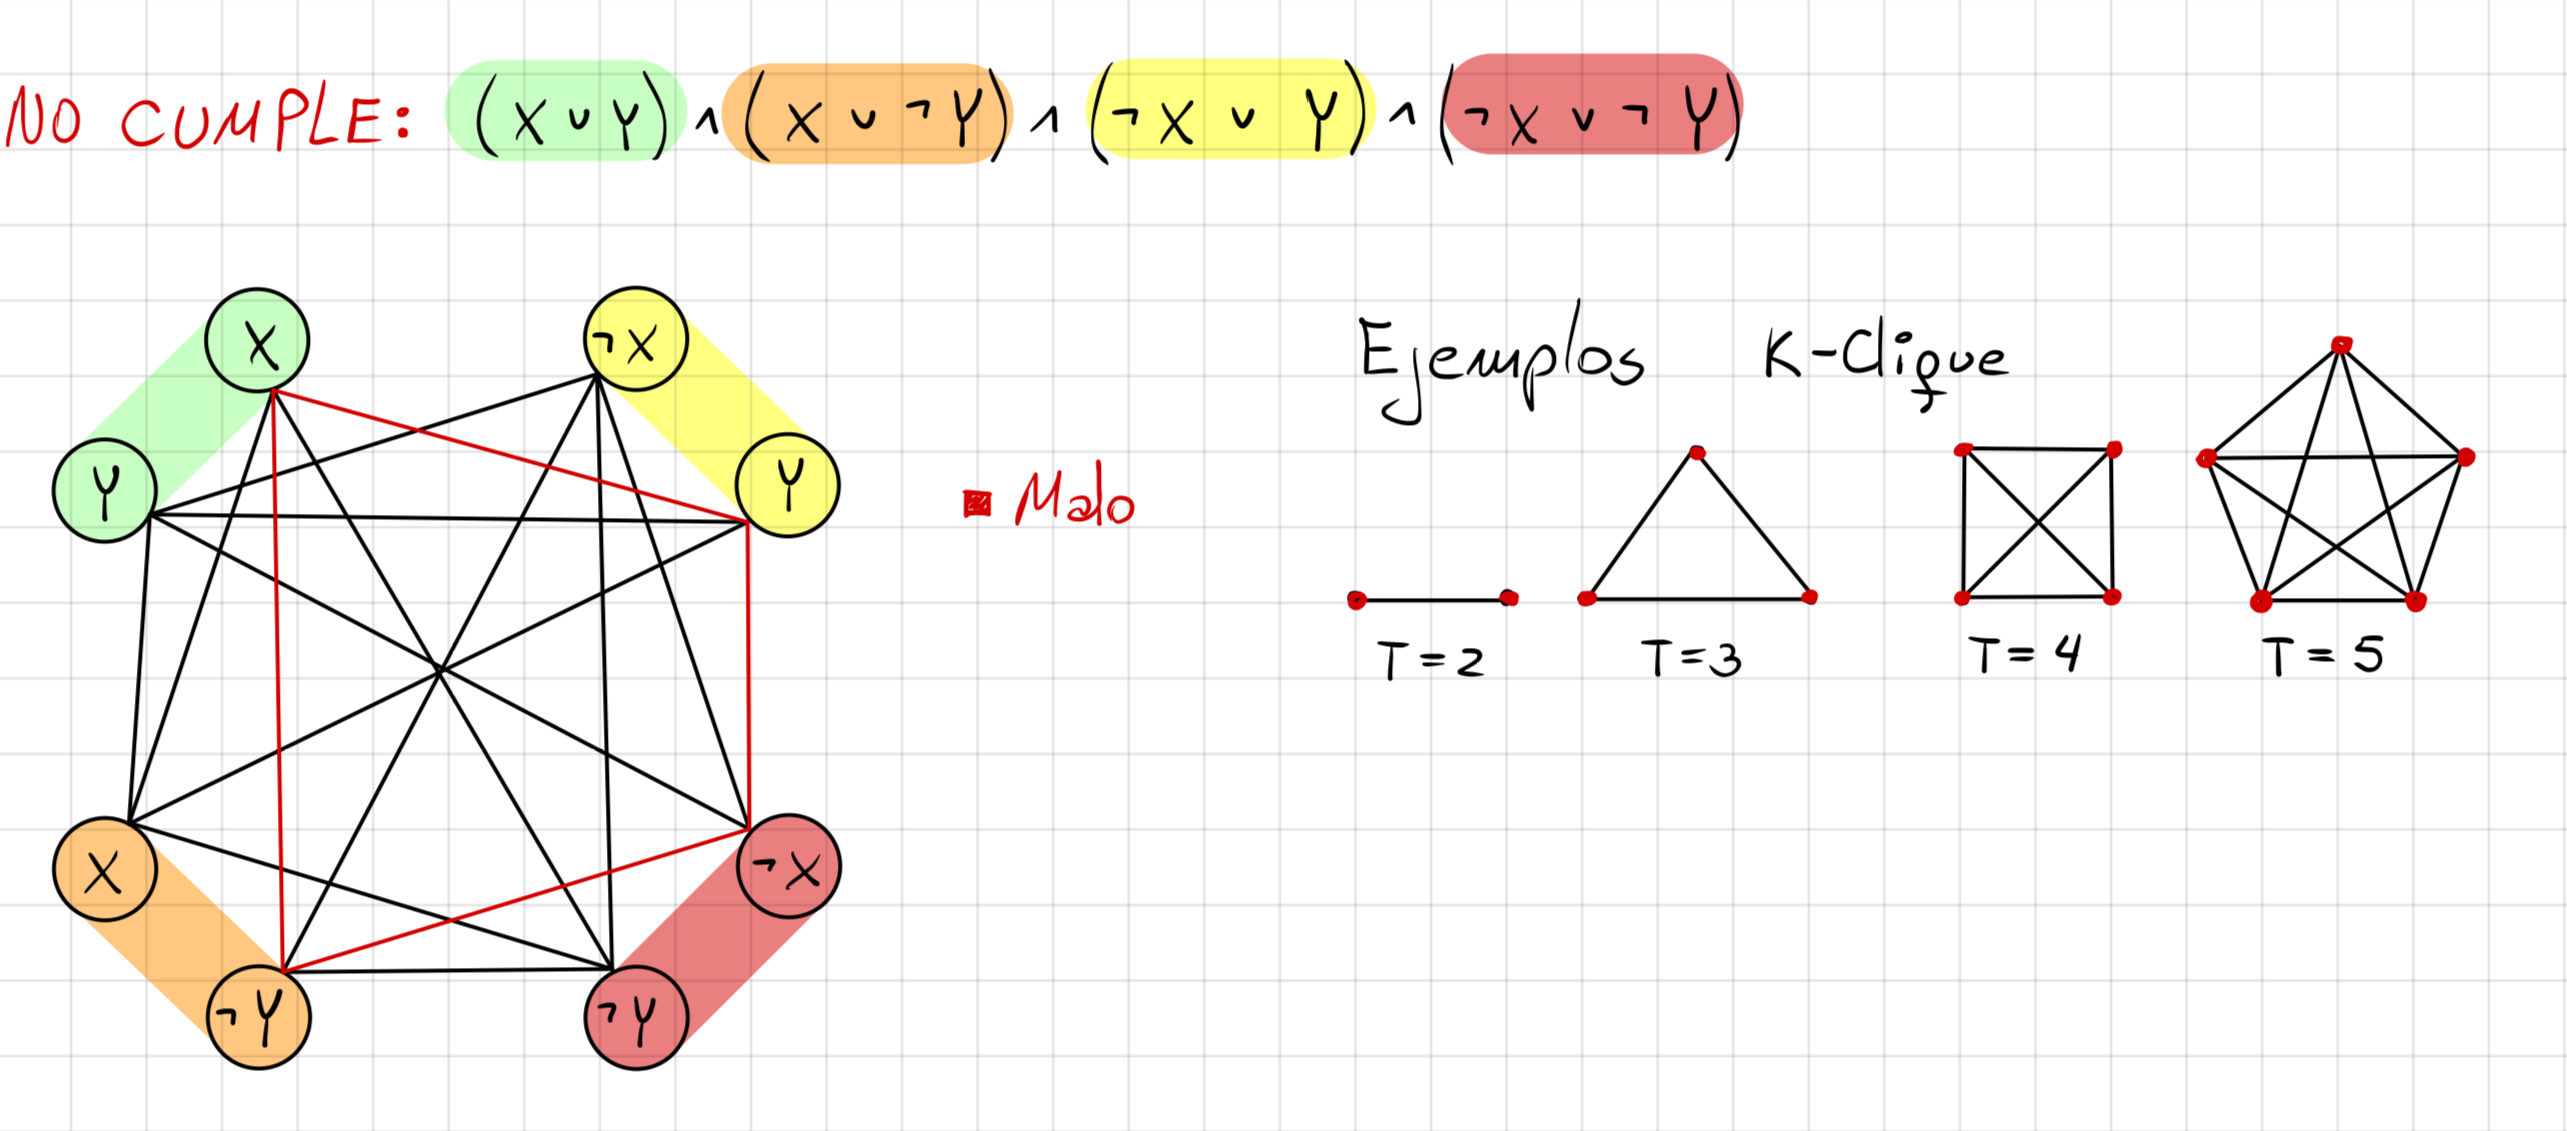
\includegraphics[scale=0.17]{img/Problema3-SATK-CliqueP2.jpg}
    \end{figure}

\end{itemize}

\section{Ejercicios:}
\subsection*{Certamen 2 G 2021}
\begin{enumerate}
    \item Sean $A$, $B$, $C$ matrices de $n \times n$. Considere el siguiente algoritmo probabilístico para saber si $A \cdot B = C$:
\begin{verbatim}
for (i = 1; i <= k; i++) {
    Generar un vector aleatorio x de n x 1 con entradas en {0 , 1}
    if (A*(Bx) != Cx)
        return false;
}
return true;
\end{verbatim}

    \textbf{Responda:}
    \begin{itemize}
        \item \textbf{a)} Tipo (MonteCarlo o las Vegas)
        
        \textbf{Respuesta:} MonteCarlo, pues el algoritmo puede mentir.
        Ejemplo:
        
        Sea A = $\begin{pmatrix} 1 & 2 \\ 3 & 4 \end{pmatrix}$, B = $\begin{pmatrix} 1 & 0 \\ 0 & 1 \end{pmatrix}$, C = $\begin{pmatrix} 0 & 2 \\ 0 & 4 \end{pmatrix}$, k = 1 y x = $\begin{pmatrix} 0 \\ 1 \end{pmatrix}$. 
        
        \begin{align*}
            A \cdot B &=^? C \\
            \begin{pmatrix} 1 & 2 \\ 3 & 4 \end{pmatrix} \cdot \begin{pmatrix} 1 & 0 \\ 0 & 1 \end{pmatrix} &=^? \begin{pmatrix} 0 & 2 \\ 0 & 4 \end{pmatrix} \\
            \begin{pmatrix} 1 & 2 \\ 3 & 4 \end{pmatrix} &\neq \begin{pmatrix} 0 & 2 \\ 0 & 4 \end{pmatrix}
        \end{align*}

        Primero:
        \begin{align*}
            A \cdot (B \cdot x) &= \begin{pmatrix} 1 & 2 \\ 3 & 4 \end{pmatrix} \cdot \left( \begin{pmatrix} 1 & 0 \\ 0 & 1 \end{pmatrix} \cdot \begin{pmatrix} 0 \\ 1 \end{pmatrix} \right)\\
            &= \begin{pmatrix} 1 & 2 \\ 3 & 4 \end{pmatrix} \cdot \begin{pmatrix} 0 \\ 1 \end{pmatrix} \\
            &= \begin{pmatrix} 2 \\ 4 \end{pmatrix}
        \end{align*}

        Luego:
        \begin{align*}
            C \cdot x &= \begin{pmatrix} 0 & 2 \\ 0 & 4 \end{pmatrix} \cdot \begin{pmatrix} 0 \\ 1 \end{pmatrix} \\
            &= \begin{pmatrix} 2 \\ 4 \end{pmatrix}
        \end{align*}

        Como $A \cdot (B \cdot x) = C \cdot x$, el algoritmo retorna true, pero la respuesta correcta es que $A \cdot B \neq C$.
        
        Por por lo tanto, el algoritmo puede mentir, por lo que es MonteCarlo.
        
        \newpage
        \item \textbf{b)} Si $k \ll n$, es más rápido este algoritmo que simplemente multiplicar $A \cdot B$ y compararlo con C? Justifique con comportamiento asintótico.
    
        \textbf{Respuesta:} Si, pues el algoritmo tiene una complejidad de $O(k \cdot n^2)$, mientras que multiplicar $A \cdot B$ y compararlo con C tiene una complejidad de $O(n^3)$.
        \\
        \\
        Pues el algoritmo tiene un ciclo que se repite k veces, y en cada iteración se multiplica una matriz de $n \times n$ con un vector de $n \times 1$, lo cual tiene una complejidad de $O(n^2)$, por lo que la complejidad del algoritmo es $O(k \cdot n^2)$.
        \\
        \\
        Mientras que multiplicar $A \cdot B$ y compararlo con C tiene una complejidad de $O(n^3)$, pues se multiplica una matriz de $n \times n$ con otra matriz de $n \times n$, lo cual tiene una complejidad de $O(n^3)$, y luego se compara con otra matriz de $n \times n$, lo cual tiene una complejidad de $O(n^2)$, por lo que la complejidad de multiplicar $A \cdot B$ y compararlo con C es $O(n^3)$.
    \end{itemize}

    \item Sea una cadena de ADN de largo $10^9$. La cantidad de adeninas en la cadena son 300 millones, timinas 200 millones, citosinas son 100 millones y guaninas el resto. Cuál es el mínimo teórico de información que posee la cadena?
    
    El mínimo teórico es la entropía, la cual se calcula de la siguiente forma:
    \begin{align*}
        h = \sum_{i=1}^{n} p_i \cdot \log_2 \left( \frac{1}{p_i} \right)
    \end{align*}

    Para calcular la entropía, primero debemos calcular la probabilidad de cada elemento, la cual se calcula de la siguiente forma:

    \begin{minipage}{0.45\textwidth}
        Para adeninas:
        \begin{align*}
            p_{a} &= \frac{300 \cdot 10^6}{10^9} \\
            &= 0,3
        \end{align*}
    \end{minipage}
    \hfill
    \begin{minipage}{0.45\textwidth}
        Para timinas:
        \begin{align*}
            p_{t} &= \frac{200 \cdot 10^6}{10^9} \\
            &= 0,2
        \end{align*}
    \end{minipage}

    \begin{minipage}{0.45\textwidth}
    Para citosinas:
    \begin{align*}
        p_{c} &= \frac{100 \cdot 10^6}{10^9} \\
        &= 0,1
    \end{align*}
    \end{minipage}
    \hfill
    \begin{minipage}{0.45\textwidth}
    Para guaninas:
    \begin{align*}
        p_{g} &= 1 - p_{a} - p_{t} - p_{c} \\
        &= 1 - 0,3 - 0,2 - 0,1 \\
        &= 0,4
    \end{align*}
    \end{minipage}

    Remplazando:
    \begin{align*}
        h &= \sum_{i=1}^{n} p_i \cdot \log_2 \left( \frac{1}{p_i} \right) \\
        &= \left( p_{a} \cdot \log_2 \left( \frac{1}{p_{a}} \right) + p_{t} \cdot \log_2 \left( \frac{1}{p_{t}} \right) + p_{c} \cdot \log_2 \left( \frac{1}{p_{c}} \right) + p_{g} \cdot \log_2 \left( \frac{1}{p_{g}} \right) \right) \\
        &= \left( 0,3 \cdot \log_2 \left( \frac{1}{0,3} \right) + 0,2 \cdot \log_2 \left( \frac{1}{0,2} \right) + 0,1 \cdot \log_2 \left( \frac{1}{0,1} \right) + 0,4 \cdot \log_2 \left( \frac{1}{0,4} \right) \right) \\
        &= \left( 0,3 \cdot \log_2 \left( \frac{10}{3} \right) + 0,2 \cdot \log_2 \left( \frac{10}{2} \right) + 0,1 \cdot \log_2 \left( \frac{10}{1} \right) + 0,4 \cdot \log_2 \left( \frac{10}{4} \right) \right) \\        
    \end{align*}

\end{enumerate}

\section*{Certamen 2 G 2017}
\begin{enumerate}
    \subsection*{Representación de un arreglo con un arreglo binario (?)}
    \item Cuál es la mejor estrategia (Voraz, dinámica, divide y vencerás o backtracking) para resolver el problema de suma cero? Justifique.
    Sea:
    \begin{align*}
        A = \left\{b_1, b_2, ..., b_n\right\}\\
        \exists S \subseteq A : \sum S = 0 \\
    \end{align*}

    Ejemplo:
    \begin{align*}
        A &= \left\{1, 2, -3, 4, 5\right\}\\
        S &= \left\{1, 2, -3\right\}\\
        \sum S &= 0\\
        S_{Bi} &= \left\{1,1,1,0,0\right\}
    \end{align*}
    
    La mejor estrategia es programación dinámica.
    \\
    \item Considere el algoritmo para el resolver el problema de las N-Reinas visto en clases, donde se elegía la permutación al azar de las reinas en el tablero (por columna) y posteriormente se hacían cambios voraces hasta conseguir el resultado deseado. Si eso no era posible, se repetia el proceso. De que tipo de algoritmo probabilístico estamos hablando? Justifique.
    
    \textbf{Respuesta:} Algoritmo de backtracking, pues se descartan soluciones intermedias que se puede determinar no llegarán a una solución.

    \item Tiene el archivo audio.mp3, que pesa 3.5MB. Suponga que tiene un sintetizador de voz y un mezclador que pueden reproducir de manera exacta el contenido del mp3,cada uno pesa 300Kb. Que puede decir respecto al Kolmogorov de audio.mp3? Justifique.
    
    \textbf{Respuesta COPILOT:} Que el Kolmogorov de audio.mp3 es aproximadamente 600Kb pues es la suma del sintetizador de voz y el mezclador, pues el Kolmogorov es el mínimo real, y el sintetizador de voz y el mezclador son programas que generan el mensaje audio.mp3.
\end{enumerate}

\newpage
\section*{Reducción Karp}
Sea: 
\begin{align*}
    EXP &= \left\{ \left( a,b,c \right) : a^b=c\right\} \\
    LOG &= \left\{ \left( x,y,z \right) : \log_y x = z\right\} \\
\end{align*}

Demuestre que $EXP \leq_p LOG$:
\begin{align*}
    \left(a,b,c\right) \overset{f}{\rightarrow} \left(x,y,z\right) \\
\end{align*}

Donde:
\begin{align*}
    f \left( a,b,c \right) = \begin{cases}
        a = y \\
        b = z \\
        c = x \\
    \end{cases} \\
\end{align*}

Recordemos que:
\begin{align*}
    \log_a c = b \Leftrightarrow a^b = c \\
\end{align*}

Sea:
\begin{align*}
    SUM &= \left\{\left(a,b,c\right):  a+b=c\right\} \\
    MULT &= \left\{\left(x,y,z\right):  x \cdot y=z\right\} \\
\end{align*}
Demuestre que $MULT \leq_p SUM$:
\begin{align*}
    \left(x,y,z\right) \overset{f}{\rightarrow} \left(a,b,c\right) \\
\end{align*}

Donde $f$:

\begin{algorithm*}[H]
    \SetKwFunction{FMain}{f}
    \SetKwProg{Fn}{Función}{:}{}
    \Fn{\FMain{}}{
        z = 0\\
        \For{: i = 1 to y}{
            Encontrar: $z' : (z, x, z')$\\
            $z \leftarrow z'$\\
        }
    }
\end{algorithm*}

\newpage
\section*{Satisfacción de Restricciones}
\begin{itemize}
    \item \textbf{Problema de Satisfacción de Restricciones (CSP):} Es un problema consistente de una tripleta $(X,D,C)$.
    \subitem $X$= Conjunto de variables.
    \subitem $D$ = Conjunto de dominios.
    \subitem $C$ = Conjunto de restricciones.
    
    \item Cada variable $x_i \in d_i$ y debe satisfacer $c_i$, el cual está formado por una relación entre elementos de $X$.
    
    \item \textbf{Ejemplo:} Problema del Caballo.
    \begin{itemize}
        \item $X = \left\{ x_1, x_2, x_3, ..., x_{64} \right\}$ donde $x_i$ es la posición del caballo en el tablero.
        
        Ejemplo: X =$\left\{ 63, 14, 37, ..., 31 \right\}$
        
        \item $D$ = $\left\{ 1, 2, 3, ..., 64 \right\}$ \quad (?)
        \item $C$ = \begin{itemize} \item Valores distintos. \item Posición en L con la casilla anterior. \{ $t[i-2][j-1]$, $t[i-2][j+1]$, $t[i-1][j+2]$, $t[i+1][j+2]$, $t[i+2][j+1]$, $t[i+2][j-1]$, $t[i+1][j-2]$, $t[i-1][j-2]$ \} \end{itemize}
        \begin{figure}[H]
            \centering
            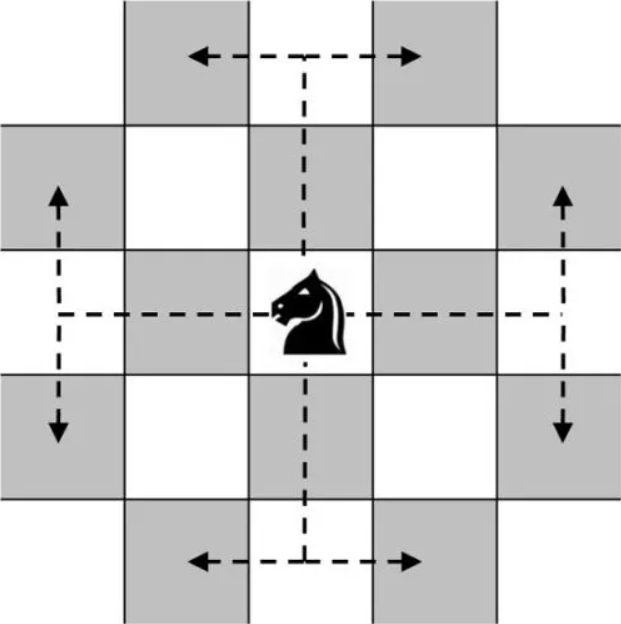
\includegraphics[scale=0.5]{img/ProblemaDelCaballo.png}
        \end{figure}
    \end{itemize}
\end{itemize}

\newpage
\section{Backtracking}
\begin{itemize}
    \item Es una meta-heurística que trata de podar el árbol de búsqueda, el cuál se va generando de manera dinámica.
    
    \item Se descartan soluciones intermedias que se puede determinar no llegarán a una solución.
    
    \item La búsqueda se hace en profundidad.

    Para realizar backtracking, necesitamos:
    \begin{enumerate}
        \item Punto de partida del árbol.
        
        \item Función de rechazo.
        
        \item Función de aceptación.
        
        \item Funciones de hijo (primero y siguiente).
        
        \item Función de Output (completar).
    \end{enumerate}
\end{itemize}

\begin{algorithm*}[H]
    % \SetAlgoLined
    \SetKwFunction{FMain}{Backtracking}
    \SetKwProg{Fn}{Función}{:}{}
    \Fn{\FMain{c}}{
        \If{reject(P,c)}{
            \KwRet\;
        }

        \If{accept(P,c)}{
            output(P,c)\;
            exit(0)\;
        }
        s = first(P,c)\;

        \While{$s \neq \land$}{
            Backtracking(s)\;
            s = next(P,s)\;
        }
    }
    \caption{PseudoCódigo Backtracking}
\end{algorithm*}

% \newpage
\subsection*{Eficiencia de backtracking}

\begin{itemize}
    \item \textbf{Función de rechazo:} Mientras más cerca de la raíz, mejor.
    
    \item \textbf{Función de aceptación:} Mientras más cerca de la raíz, mejor.
    
    \item \textbf{Funciones de hijo (primero y siguiente):} Mientras más restrictiva, mejor.
    
    \item \textbf{Función de Output (completar):} Mientras más eficiente, mejor.
\end{itemize}

\subsection*{Cuando usar backtracking}
\begin{itemize}
    \item BackTracking está considerado para resolver Problemas de Satisfacción de Restricciones (CSP).
    Éste se define como los problemas consistentes de una tripleta $(X,D,C)$.
    \subitem $X$= Conjunto de variables.
    \subitem $D$ = Conjunto de dominios.
    \subitem $C$ = Conjunto de restricciones.
    
    \item Cada variable $x_i \in d_i$ y debe satisfacer $c_i$, el cual está formado por una relación entre elementos de $X$.
    
\end{itemize}


\subsection*{Ejemplos de problemas CSP}

\begin{tcolorbox}[colback=blue!4!white,colframe=blue!75!black,title=Aritmética Verbal]
    Dado un problema de aritmética verbal, encontrar la solución.
\end{tcolorbox}

\begin{tcolorbox}[colback=blue!4!white,colframe=blue!75!black,title=Coloración de mapas]
    Dado un mapa, colorear las regiones de tal forma que dos regiones adyacentes no tengan el mismo color.
\end{tcolorbox}

\begin{tcolorbox}[colback=blue!4!white,colframe=blue!75!black,title=Crucigramas]
    Dado un crucigrama, encontrar las palabras que lo completan.
\end{tcolorbox}

\begin{tcolorbox}[colback=blue!4!white,colframe=blue!75!black,title=Sudoku]
    Dado un tablero de $9 \times 9$, colocar los números del 1 al 9 de tal forma que no se repitan en la misma fila, columna o submatriz de $3 \times 3$.
\end{tcolorbox}

\begin{tcolorbox}[colback=blue!4!white,colframe=blue!75!black,title=Problema de las $n$ reinas]
    Dado un tablero de $n \times n$, colocar $n$ reinas de tal forma que no se ataquen entre ellas.
\end{tcolorbox}

\newpage

\section{Algoritmos Probabilísticos}
\begin{itemize}
    \item Los algoritmos probabilísticos son aquellos que introducen elementos al azar dentro de su lógica.
    \item Puede que el tiempo, la memoria o la respuesta sean afectados positivamente (o negativa con baja probabilidad) por el azar.
\end{itemize}

\subsection*{Tipos}
\begin{itemize}
    \item Algoritmos Numéricos.
    \begin{itemize}
        \item Estos algoritmos dan una respuesta aproximada al problema que se quiere resolver.

        \item Su precisión mejora conforme se realizan más ciclos de iteración.
    \end{itemize}

    \item \textbf{Algoritmos Monte Carlo} (Puede mentir).
    \begin{itemize}
        \item Se utilizan cuando no existen formas eficientes de resolver un problema de otra manera.

        \item \hl{Estos algoritmos dan la respuesta exacta, pero puede dar una solución errada, con probabilidad baja.}

        \item Mientras más larga la ejecución, mayor es la probabilidad de que la respuesta se la correcta.
        
        Se le dice a un algoritmo tipo Monte Carlo p-correcto si:
        \begin{itemize}
            \item La solución regresada es correcta con probabilidad p>0,5, no importando el dato de entrada.
            \item p puede depender del tamaño de la entrada, pero no de los datos de la entrada.
        \end{itemize}

    \end{itemize}
    
    \item \textbf{Algoritmos Las Vegas} (No miente, dice que no puede dar la respuesta correcta).
    \begin{itemize}
        \item El algoritmo tipo Las Vegas funciona similar a Monte Carlo, pero cuando no puede dar una respuesta correcta, lo admite.
        
        Se distinguen 2 sub-tipos en general:
        \begin{itemize}
            \item Siempre encuentra una solución correcta. Si el azar no beneficia a la ejecución, esta tomará más tiempo.
            \item \hl{A veces no es capaz de dar una solución, lo cual admite.}
        \end{itemize}
    \end{itemize}
\end{itemize}

\section{Algoritmos Genéticos}
\begin{itemize}
    \item Algoritmo genético es una metaheurística que se inspira en la evolución y selección natural para resolver problemas de optimización.
    
    \item En términos coloquiales, genera una población inicial y la hace evolucionar miles o millones de años, para finalmente elegir al individuo más fuerte.
    
    \newpage
    En términos generales, los tópicos ligados a un algoritmo genético son los siguientes:
    \begin{enumerate}
        \item \textbf{Población Inicial:} La Población Inicial consta de soluciones (ya sean parciales y/o totales).

        \item \textbf{Función de aptitud:}La Fitness Function o Función de Aptitud nos dice que tan apta es la solución para el problema.
        
        \item \textbf{Algoritmo de combinación (sexo):} Básicamente acá es que los individuos con mejor fitness tienen mayores posibilidades de procrear.

        \item \textbf{Algoritmo y tasa de Mutación:} Con alguna probabilidad (generalmente muy baja), cada bit de hijos puede cambiar.
        \begin{itemize}
            \item Mutación bit por string.
            
            \item Flip.
            
            \item Límite (para números).
            
            \item No uniforme.
            
            \item Uniforme.
            
            \item Gausiano.
            
            \item Shrink.
        \end{itemize}
        \item \textbf{Selección:} Hay varias versiones sobre supervivencia a la siguiente generación. Una común es que sobrevivan los mejores (siempre mismo tamaño).

    \end{enumerate}

\end{itemize}

\section{Búsqueda Informada (Heurística)}
La búsqueda no informada trata ciegamente de encontrar una solución.
\begin{itemize}
    \item Fuerte: Se usa heurística para tratar de resolver el problema lo mejor posible, pero no se asegura la solución.
    \item Débil: Heurística se conjuga con un método riguroso para llegar a la mejor solución. Muchas veces sigue siendo infactible de resolver en el peor caso.
\end{itemize}

\section{Complejidad Computacional}
\begin{itemize}
    \item La complejidad computacional trata sobre clasificación de problemas.
    \subitem Dificultad inherente.
    \subitem Clases de complejidad y sus relaciones.
    
    \item Mide Tiempo y Espacio utilizando modelos de cómputo.
\end{itemize}

\section{Teoría Algorítmica de la Información}

\section{Dureza, Completitud y Reducciones}

\newpage
\section{Clases de Complejidad}
COPILOT
\begin{itemize}
    \item \textbf{Problemas NP:} Problemas que pueden ser resueltos en tiempo polinomial por una máquina de Turing no determinista.
    \item \textbf{Problemas NP-Duros:} Problemas que son al menos tan difíciles como los problemas NP.
    \item \textbf{Problemas NP-Completos:} Problemas que son NP y NP-Duros.
    \item \textbf{Problemas P:} Problemas que pueden ser resueltos en tiempo polinomial por una máquina de Turing determinista.
    \item \textbf{Problemas EXPTIME:} Problemas que pueden ser resueltos en tiempo exponencial por una máquina de Turing determinista.
    \item \textbf{Problemas EXPSPACE:} Problemas que pueden ser resueltos en espacio exponencial por una máquina de Turing determinista.
    \item \textbf{Problemas PSPACE:} Problemas que pueden ser resueltos en espacio polinomial por una máquina de Turing determinista.
    \item \textbf{Problemas EXP:} Problemas que pueden ser resueltos en tiempo y espacio exponencial por una máquina de Turing determinista.
    \item \textbf{Problemas LOGSPACE:} Problemas que pueden ser resueltos en espacio logarítmico por una máquina de Turing determinista.
    \item \textbf{Problemas L:} Problemas que pueden ser resueltos en tiempo logarítmico por una máquina de Turing determinista.
    \item \textbf{Problemas NL:} Problemas que pueden ser resueltos en tiempo logarítmico por una máquina de Turing no determinista.
    \item \textbf{Problemas co-NP:} Problemas cuyas respuestas negativas pueden ser verificadas en tiempo polinomial por una máquina de Turing determinista.
\end{itemize}

\section{Problemas NP-Completos}


\end{document}